\documentclass[a4paper,11pt]{article}
\usepackage[utf8]{inputenc}
\usepackage[italian]{babel}
\usepackage{amsmath}
\usepackage{amsfonts}
\usepackage{amssymb}
\usepackage{physics}
\usepackage{graphicx}
\usepackage{subfig}
\usepackage{hyperref}
\usepackage{parskip}
\usepackage{tabu, wrapfig}
\usepackage[italiano, ruled]{algorithm2e}
\usepackage[left=1in, right=1in]{geometry}

%opening
\title{Simulazione numerica di una particella libera sul cerchio nel limite di bassa temperatura}
\author{Rocco Francesco Basta}
\date{}

\newcommand{\avg}[1]{\langle {#1} \rangle}
\newcommand{\code}[1]{\texttt{#1}}

\begin{document}

\maketitle

\begin{abstract}
    Lo studio numerico del sistema quantistico di una particella libera sul cerchio presenta particolari difficoltà dovute alla peculiare topologia del sistema. Sono stati messi a confronto tre diversi metodi per misurare la suscettività topologica del sistema nel limite di bassa temperatura: un algoritmo Metropolis locale, un algoritmo non locale e infine un metodo basato sullo studio di sottovolumi (\emph{slab}) del cammino totale. Infine, il metodo non locale è stato applicato allo studio dello spettro del sistema. 
\end{abstract}

\section{Introduzione}

    Il sistema è composto da una particella di massa $m$, libera di muoversi su un cerchio di raggio $R$. L'hamiltoniana del sistema è
    %
    \begin{equation}
        H = \frac{p^2}{2m} \quad \quad p = \frac{\hbar}{i} \partial_x
    \end{equation}
    %
    dove $x \in [0, L = 2\pi R)$. D'ora in poi, poniamo $\hbar = 1$.
    Per effettuare la simulazione, passiamo a quantità adimensionali:
    %
    \begin{equation}
        x \equiv L\left(\hat{x} + \frac{1}{ 2} \right) \quad \quad
        p \equiv \frac{\hat{p}}{L} \quad \quad 
        H \equiv \frac{1}{mL^2} \hat{H}
    \end{equation}
    %
    \begin{equation}
        \hat{H} = \frac{1}{2} \hat{p}^2
    \end{equation}
    %
    Il sistema è caratterizzato da uno spettro discreto in energia. La funzione di partizione può essere quindi calcolata come traccia sulla base degli autostati di $\hat{H}$:
    %
    \begin{equation}
        Z = \Tr e^{-\beta H} = \Tr e^{-\hat{\beta} \hat{H}}
    \end{equation}
    %
    dove $\hat{\beta} = \beta / mL^2 = \frac{1/mL^2}{kT}$ è il rapporto fra la scala di energia caratteristica del sistema (a meno di costanti) e la scala di energia termica.
    
    Analogamente, possiamo scrivere l'azione euclidea:
    %
    \begin{equation}
        S_E = \int_0^\beta d\tau \, \frac{1}{2} m \left(\frac{dx}{d\tau}\right)^2 = \int_0^{\hat{\beta}} d\tau \, \frac{1}{2} \left( \frac{d\hat{x}}{d\tau}\right)^2
    \end{equation}
    %
    Possiamo quindi riscrivere la funzione di partizione in termini dell'integrale sui cammini chiusi $\hat{x}(\tau): [0, \hat{\beta}] \to [-1/2, 1/2)$:
    
    \begin{equation}
        Z = \mathcal{N} \int_{\hat{x}(0) = \hat{x}(\hat{\beta})} \mathcal{D}\hat{x}(\tau) \, \,e^{-S_E}
    \end{equation}

    \subsection{Campo magnetico uniforme}
    In presenza di un campo magnetico uniforme, l'azione euclidea diventa
    %
    \begin{equation}
        S^{(\theta)}_E = S^{(0)}_E + i\theta Q
    \end{equation}
    %
    dove $Q = \int_0^{\hat{\beta}} d\tau \, ({d\hat{x}} / {d\tau})$ è la \emph{carica topologica}, data dal numero di avvolgimenti del cammino intorno al cerchio, mentre $\theta = qB\pi R^2$ è un termine dipendente dal campo magnetico esterno. 
    
    Il fattore $i$ del secondo termine viene dalla continuazione analitica al tempo immaginario dell'azione ottenuta mediante l'accoppiamento minimale, e porta ad una distribuzione di probabilità dei cammini che non è più definita positiva (né reale). 
    
    Possiamo scrivere l'energia libera del sistema, in termini di $\theta$, come
    
    \begin{equation}
        F(\theta) = F^{(0)} + \sum_{k=1}^{\infty} \frac{F^{(2k)}}{(2k)!} \theta^{2k}
    \end{equation}
    %
    dove abbiamo usato che $F(\theta)$ deve essere simmetrica per parità. Il termine $F^{(1)} \equiv \chi$ è detto \emph{suscettività topologica}.
    
    Per evitare il problema del segno causato dal termine $iQ\theta$, conviene determinare $\chi$ simulando il sistema per $\theta = 0$, sfruttando la relazione
    
    \begin{equation}
        \chi \equiv \frac{\partial^2 F}{\partial \theta^2} \bigg\rvert_{\theta = 0} = \frac{\avg{Q^2}}{
        \hat{\beta}}
    \end{equation}
    
    Nel limite di bassa temperatura, la distribuzione di $Q$ è gaussiana, e si ha $\chi \to 1$, mentre gli altri termini $F^{(2k, k \neq 1)} \to 0$.
    
    Nel limite di alta temperatura, invece, si ha $\chi \simeq \hat{\beta}^{-1} e^{-\frac{1}{2\hat{\beta}}}$. Tuttavia, lo studio numerico di questo regime presenta difficoltà ulteriori: la distribuzione di probabilità della carica topologica diventa fortemente piccata in $Q = 0$. Questo impedisce, di fatto, di utilizzare i metodi che tratteremo per lo studio della suscettività topologica ad alta temperatura.
    
    D'ora in poi, verranno tralasciati i segni di circonflesso per le quantità adimensionali. Questo è equivalente a porre $L=1, m = 1 \implies mL^2 = 1$, e a considerare $x \in [-1/2, 1/2)$.
    
    \subsection{Spettro}
    
    Possiamo definire degli operatori di \emph{salita} e \emph{discesa} nell'autovalore di $p$:
    
    \begin{eqnarray}
        a = e^{-i2\pi x} \quad a^\dagger = e^{i2\pi x} \\
        \left[p, a \right] = - 2\pi a \quad \left[p, a^\dagger \right] = 2 \pi a^\dagger
    \end{eqnarray}

    Utilizzeremo questi due operatori per costruire le funzioni di correlazione che andremo a studiare.
    
    Lo spettro del sistema è dato da
    %
    \begin{equation}
        E_n = 2\pi^2 n^2 \quad n \in \mathbb{Z}
    \end{equation}
    %
    dove a ogni $n \in \mathbb{Z}$ corrisponde un autostato di $p, H$. Ogni livello energetico ha quindi degenerazione 2.
    
    
    

    
\section{Algoritmi}

    Una volta passati a quantità adimensionali, il cammino $[0, \beta]$ è stato diviso in $N$ intervalli di ampiezza $\eta$. L'azione discretizzata ha la seguente forma:
    
    \begin{equation}
        S_{E,L} = \frac{1}{2\eta} \sum_i d(x_{i+1}, x_{i})^2
    \end{equation}
    
    dove $d(x,y) = [x - y]_{S^1}$ è la distanza con segno fra i due punti. Per semplicità di notazione, le condizioni periodiche sono implicite nella scrittura: con $x_{i+k}$ indichiamo $x_{(i + k) \mathrm{mod} N}$.
    
    Il limite del continuo a temperatura fissata si ottiene mandando $N \to \infty$, $\eta \to 0$ con $N\eta = \beta$.
    
    
    \subsection{Algoritmo locale}
    
    Il primo algoritmo utilizzato è un semplice algoritmo Metropolis in cui ogni sito viene aggiornato, sequenzialmente, spostandolo in una posizione $x_i \to x^P_i \in [x - \delta, x + \delta]$.
    
    Come vedremo, nel limite del continuo questo algoritmo ha difficoltà a passare da un cammino con carica topologica $Q$ ad un altro con carica $Q' \neq Q$. Questo porta a un congelamento dei modi topologici, e a un aumento esponenziale dei tempi di autocorrelazione associati alla carica topologica (\emph{critical slowing down esponenziale}).
    
    \begin{algorithm}[H]
    Cammino x[N]\;
    \For{$i = 0$; $i < N$}{
        estraggo $x_i^p \in [x_i - \delta, x_i + \delta]$ con distribuzione uniforme\;
        \tcp{Test di Metropolis}
        r = $\exp(-\Delta S_{E,L})$\;
        \eIf{$r \geq 1$}{
            accetto $x_i = x_i^p$ 
        }{
            accetto $x_i = x_i^p$ con probabilità r \;
        }
    }
    \caption{Algoritmo locale}
    \label{alg:local}
    \end{algorithm}
    
    \subsection{Algoritmo non-locale}
    
    Il secondo algoritmo utilizzato aggiunge all'algoritmo locale una mossa aggiuntiva: cerco due punti in cui $d(x_i, x_j) \sim 1/2$, ovvero il cammino si avvolge per mezzo giro (o 3/2, 5/2...). A questo punto, tento di ``ribaltare'' la sezione di cammino compresa tra i due punti attorno al punto iniziale, con un test di Metropolis. Se il cambiamento viene accettato, $Q$ varia di un numero intero. Questo permette di passare più facilmente da un modo topologico all'altro.

    \begin{algorithm}[H]
    Cammino x[N]\;
    compio una spazzata su x[N] con l'algoritmo locale\;
    scelgo $i < N$\;
    cerco $k < N$ tale che $| d(x_{i+k}, x_i) - 1/2| < \epsilon$\;
    \eIf {$\nexists k$}{tentativo fallito}{
    \tcp{Rifletto attorno a $x_i$ la sezione di cammino compresa tra $x_i$ e $x_{i+k}$}
    $(x^p_{i+1}, \, \dots \, ,x^p_{i+k}) = 2 x_i - (x_{i+1}, \, \dots \,  , x_{i+k}) $\;
    \tcp{Test di Metropolis, esattamente come nell'algoritmo locale}
    r = $\exp(-\Delta S_{E,L})$\;
    \eIf{$r \geq 1$}{
            accetto $(x_{i+1}, \, \dots \, ,x_{i+k}) = (x^p_{i+1}, \, \dots \, ,x^p_{i+k}) $ \;
        }{
            accetto $(x_{i+1}, \, \dots \, ,x_{i+k}) = (x^p_{i+1}, \, \dots \, ,x^p_{i+k}) $ con probabilità r \;
        }
    }
    \caption{Algoritmo non-locale}
    \label{alg:tailor}
    \end{algorithm}
    
    \subsection{Slab method}
    
    Un metodo alternativo per calcolare la suscettività topologica è il cosiddetto \emph{slab method}. Si basa sull'algoritmo Metropolis locale, ed è generalizzabile a sistemi per cui non è stato trovato un algoritmo che risolva il congelamento dei modi topologici.
    
    L'idea è quella di considerare la carica topologica $Q_x$ calcolata non su tutto il cammino $[0, \beta]$, ma su una frazione $[0, x\beta]$, con $x \in [0,1]$. In generale, $Q_x \not\in \mathbb{Z}$ .
    
    Se l'algoritmo locale è congelato sul modo $Q = 0$, allora la probabilità di avere un certo valore di $Q_x$ è
    
    \begin{equation}
        p_x (Q_x) \times p_{1-x} (- Q_x) 
    \end{equation}

    Se la distribuzione $p_x (Q_x)$ è gaussiana, si può mostrare che, con $\chi_x \equiv \avg{Q_x^2}/\beta$, 
    
    \begin{equation}
        \chi_x = x(1-x) \chi
    \end{equation}

    
    Possiamo quindi ottenere $\chi$ da un fit.
    
    \section{Simulazioni numeriche}
    
    Sono state effettuate alcune simulazioni con $\beta = 5, 10, 15$, $N$ compreso tra 100 e 1500, usando l'algoritmo locale e quello non locale, con condizioni iniziali fissate a 0. Per ogni simulazione, sono state prese $10^6$ misure, una ogni $10$ spazzate. Le prime $10^5$ sono state scartate per termalizzazione. Il generatore di numeri pseudo-casuali utilizzato è \code{RAN2}\footnote{In particolare, è una variante adattata a generare \code{double}, estratta dal codice di Athena++, Princeton University, disponibile all'indirizzo \url{https://github.com/PrincetonUniversity/athena-public-version/blob/master/src/utils/ran2.cpp}, con un'interfaccia lievemente riadattata.}. Si è avuta particolare cura nell'effettuare le simulazioni con seed diversi, in modo da avere simulazioni indipendenti.
    
    Il tempo di autocorrelazione $\tau_\chi$ è stato determinato confrontando la stima dell'errore \emph{naïve}, ottenuta trascurando l'autocorrelazione dei dati, con quella ottenuta dal blocking. Ricordiamo che
    
    \begin{equation}
        \sigma^2_{\chi \text{, corretta}} = 2 \tau_\chi \sigma^2_{\chi \text{, naïve}}
    \end{equation}

    
    \subsection{Critical slowing down esponenziale}
    
    \begin{figure}[hptb]
        \centering
        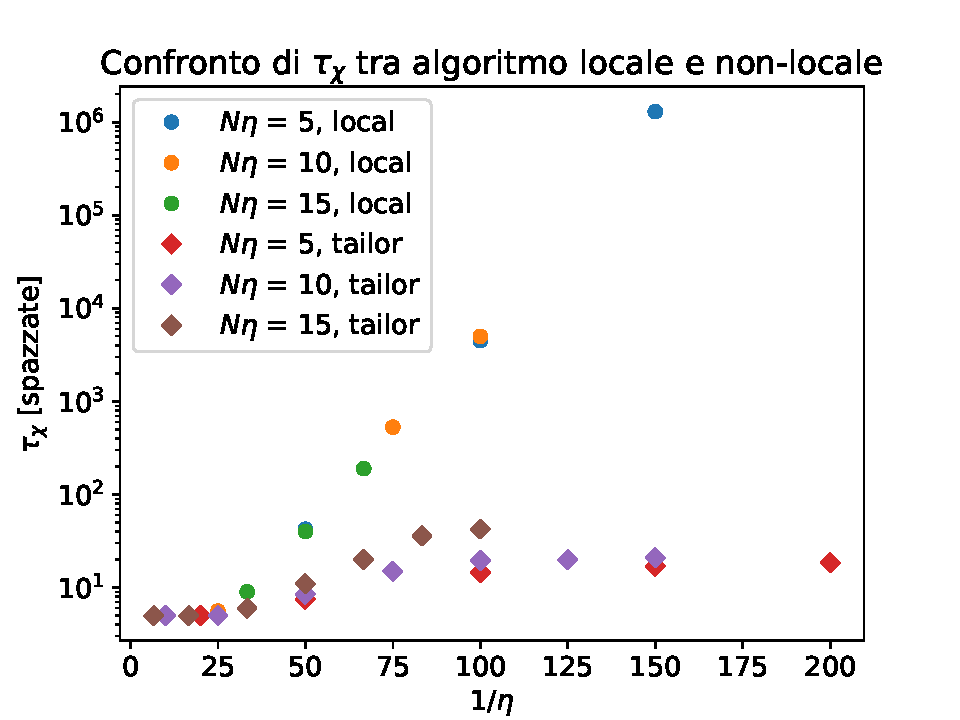
\includegraphics[width=10cm]{figure/csd_autocorr.pdf}
        \caption{Andamento del tempo di autocorrelazione $\tau_\chi$ della suscettività topologica nelle varie simulazioni effettuate. La ``coda'' per $N \to 0$ è dovuta al fatto che l'unità minima di tempo è data da 10 spazzate.}
        \label{fig:csd_autocorr}
    \end{figure}

    
    In figura \ref{fig:csd_autocorr} sono riportati i tempi di autocorrelazione di $\chi$ nelle varie simulazioni. Osserviamo che, qualitativamente, i valori di $\tau_\chi$ ottenuti dalle simulazioni con l'algoritmo locale si dispongono su un andamento grossomodo esponenziale, mentre quelli ottenuti dall'algoritmo non-locale sembrano ``saturare'' ad un valore dipendente da $\beta$. Questa non è assolutamente un'analisi rigorosa, ma si può già vedere come l'algoritmo non-locale risolva in maniera efficiente il problema del critical slowing down esponenziale.
    
    \begin{figure}[hptb]
        \centering
        \subfloat{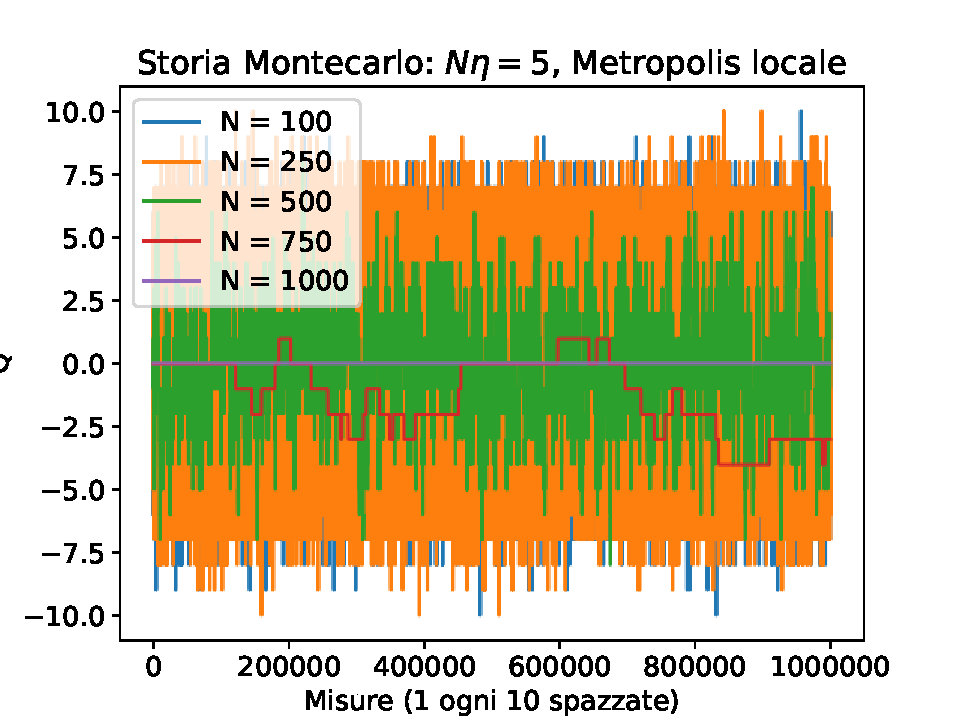
\includegraphics[width=0.5\textwidth]{figure/csd_plot_local_5.pdf}}
        \subfloat{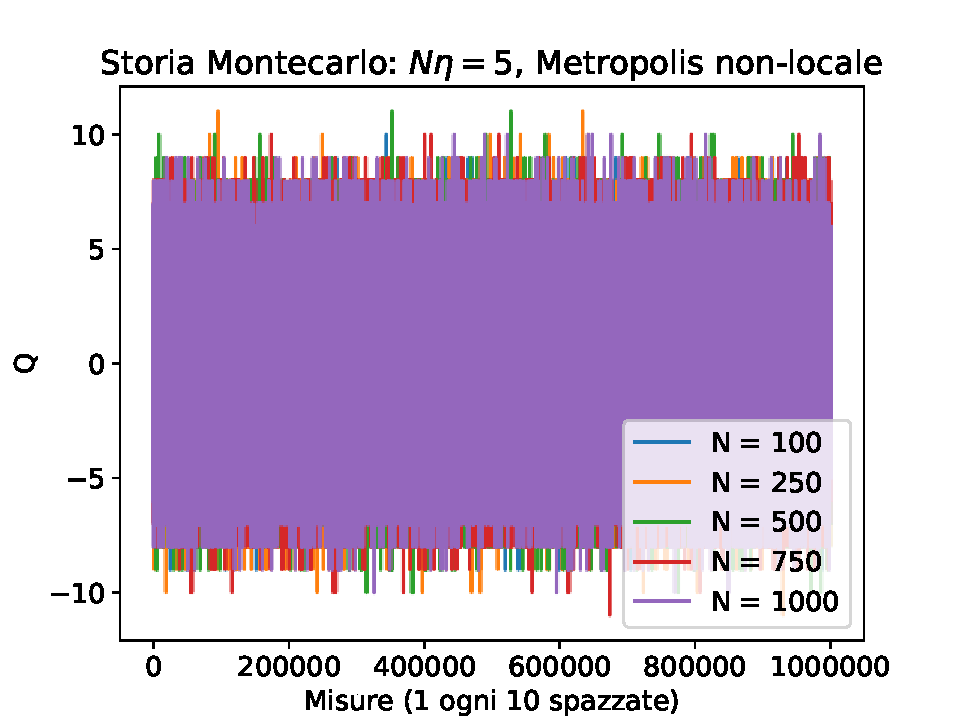
\includegraphics[width=0.5\textwidth]{figure/csd_plot_tailor_5.pdf}}
        \caption{Congelamento dei modi topologici del sistema per $N\eta = 5$ al variare di N. Confronto con l'algoritmo non-locale.}
        \label{fig:csd_topfreezing}
    \end{figure}
    
    In figura \ref{fig:csd_topfreezing} possiamo vedere il confronto tra le storie Monte Carlo delle simulazioni fatte con l'algoritmo locale e l'algoritmo non-locale, a $\beta = 5$. Notiamo che, con l'algoritmo locale, la carica topologica tende a fluttuare meno già per $N = 500$. Per $N = 750$, la carica topologica cambia poche decine di volte in $10^6$ misure, mentre per $N = 1000$ è completamente congelata a $Q = 0$. Nelle simulazioni fatte con l'algoritmo non locale, invece, il problema è completamente risolto: in tutte le simulazioni effettuate, $Q$ ``fluttua'' allo stesso modo.
    
    \subsection{Misura della suscettività topologica}
    
    \begin{wraptable}{r}{5.5cm}
        \centering
        \begin{tabular}{c c c} \hline
            $\beta$   & $\chi_\beta$    & $\chi^2$ / ndof \\ \hline
            5      & 0.9990(18)    & 0.78 \\
            10     & 0.9982(20)             & 0.47 \\
            15     & 1.0027(39)             & 2 \\ \hline
            
        \end{tabular} 
        \caption{Misura della suscettività topologica per $\beta = 5, 10, 15$}
        \label{tab:top_tailor}
    \end{wraptable}
    

    Queste simulazioni sono state utilizzate per determinare la suscettività topologica del sistema per $\beta = 5, 10, 15$. Il valore teorico da confrontare è $\chi \to 1$ per $\beta \gg 1$.
    
    Il limite al continuo è stato effettuato con un fit numerico alla funzione $\chi_\beta(\eta) = \chi_\beta + b\eta^2$, in modo da estrarre la misura della suscettività $\chi_\beta$ a temperatura $\beta$.
    
    I valori ottenuti sono riportati in tabella \ref{tab:top_tailor}, e i rispettivi fit sono riportati in figura \ref{fig:top_tailor}. Sono tutti compatibili (entro $1\sigma$!) con il valore atteso per $\beta \gg 1$.

    \begin{figure}[p]
        \centering
        \subfloat[$\beta = 5$, $\chi^2 / \mathrm{ndof} \simeq 0.78$]{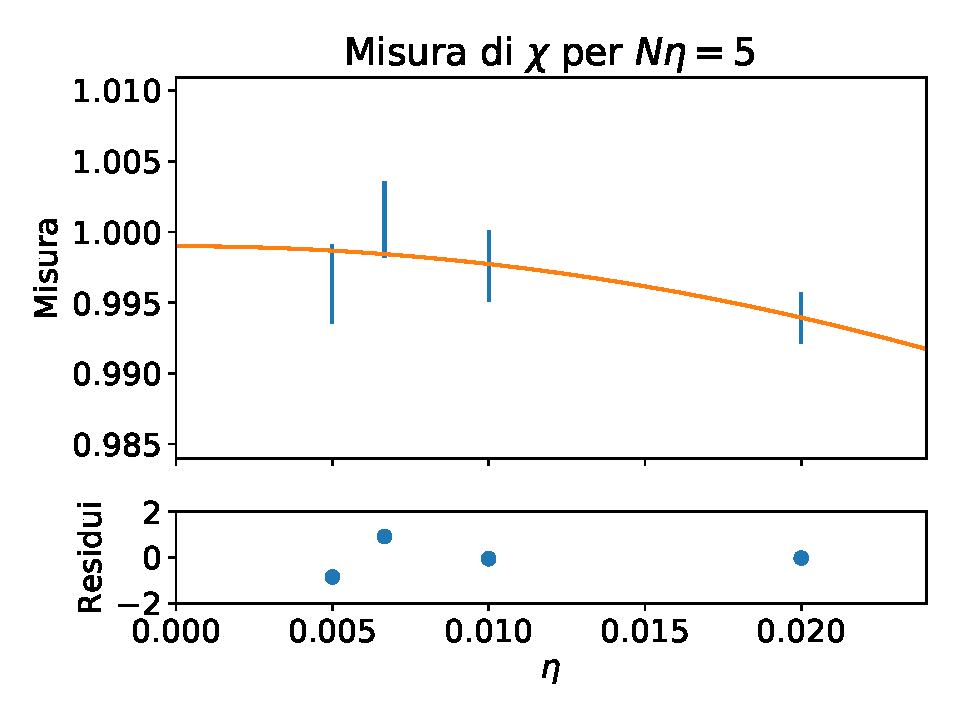
\includegraphics[width=0.5\textwidth]{figure/continuum_fit_tailor_5.pdf}}
        \subfloat[$\beta = 10$, $\chi^2 / \mathrm{ndof} \simeq 0.47$]{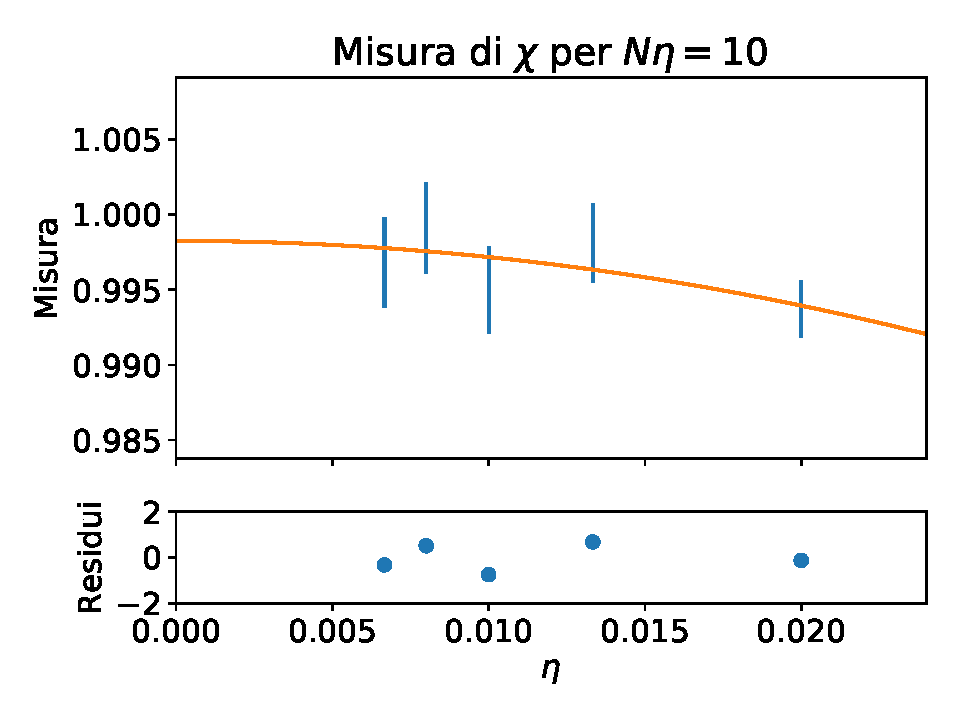
\includegraphics[width=0.5\textwidth]{figure/continuum_fit_tailor_10.pdf}}\\
        \subfloat[$\beta = 15$, $\chi^2 / \mathrm{ndof} \simeq 2$]{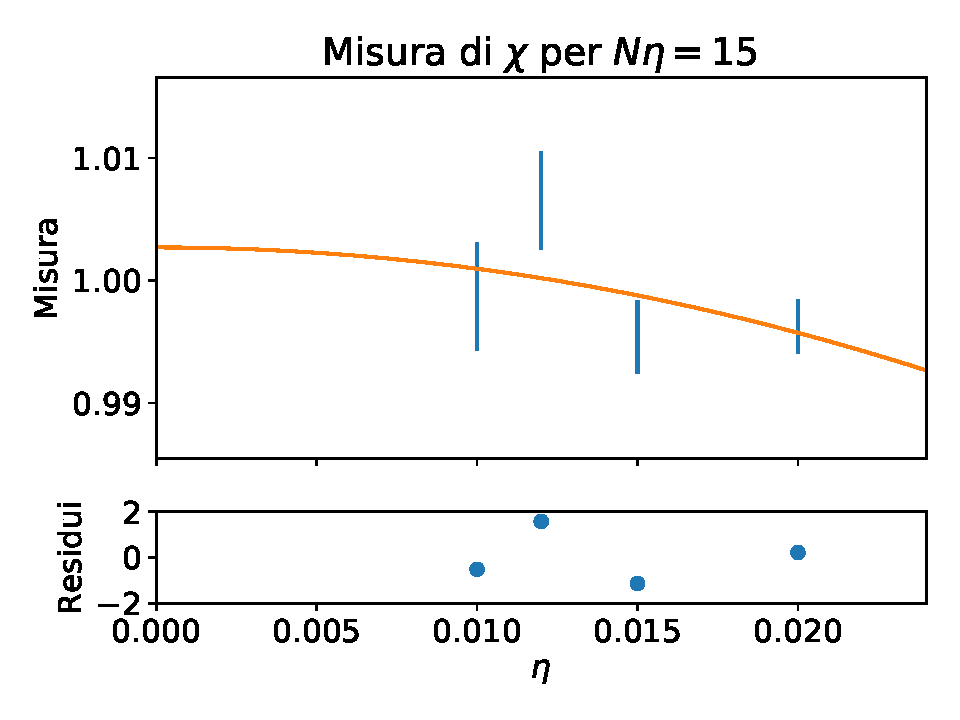
\includegraphics[width=0.5\textwidth]{figure/continuum_fit_tailor_15.pdf}}
        \caption{Misura della suscettività topologica $\chi$ per $\beta = 5,10,15$. Per ogni fit, sono riportati in basso i residui normalizzati $R = (\chi - \chi_{fit})/d\chi$.}
        \label{fig:top_tailor}     
    \end{figure}
    %
    \begin{wraptable}{r}{5.5cm}
        \centering
        \begin{tabular}{c c c} \hline
            $N$   & $\chi_{N, \beta}$    & $\chi^2$ / ndof \\ \hline
            1050    & 1.036(22)    & 1.9 \\
            1150    & 1.032(21)    & 0.39 \\
            1250    & 0.988(23)    & 1.25 \\
            1350    & 1.000(24)    & 1.50 \\
            1500    & 1.058(30)    & 0.15 \\ \hline
            $N \to \infty$ & 1.000(48) & 1.21 \\ \hline
            
        \end{tabular}
        \caption{Misura di $\chi$ per $\beta = 5$ con lo slab method}
        \label{tab:top_slab}
    \end{wraptable}
    %
    La stessa misura (solo per $\beta = 5$) è stata effettuata con lo slab method. Le simulazioni sono state effettuate per $N = 1050, 1150, 1250, 1350, 1500$ e per $x = 0.1, 0.2, 0.3, 0.4, 0.5$, prendendo $10^6$ misure, una ogni $10^2$ spazzate. Le simulazioni per ogni coppia $(N, x)$ sono fra loro indipendenti.
    
    È stato necessario spingersi a $N$ più grandi, in modo da essere sicuri che l'algoritmo fosse bloccato nel solo settore topologico $Q = 0$. Questo, insieme al fatto che per ogni $(N, \beta)$ sono state fatte più simulazioni variando $x$, ha reso lo sforzo numerico necessario decisamente maggiore rispetto al metodo non-locale.
    
    I risultati delle simulazioni, insieme al valore ottenuto dal limite del continuo, sono riportati in tabella \ref{tab:top_slab} e nella figura \ref{fig:top_slab}. La misura è in ottimo accordo con la misura analoga effettuata con il metodo non-locale e con il valore teorico.
    
    \begin{figure}[htp]
        \centering
        \subfloat[$N = 1050$]{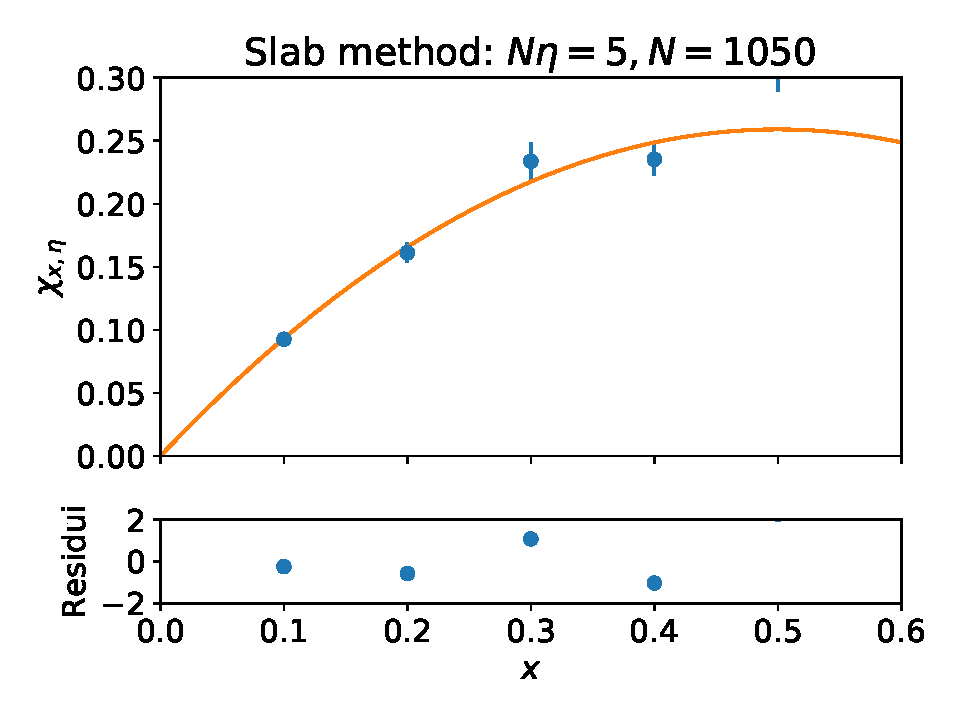
\includegraphics[width=0.5\textwidth]{figure/slab_fit_5_1050.pdf}}
        \subfloat[$N = 1150$]{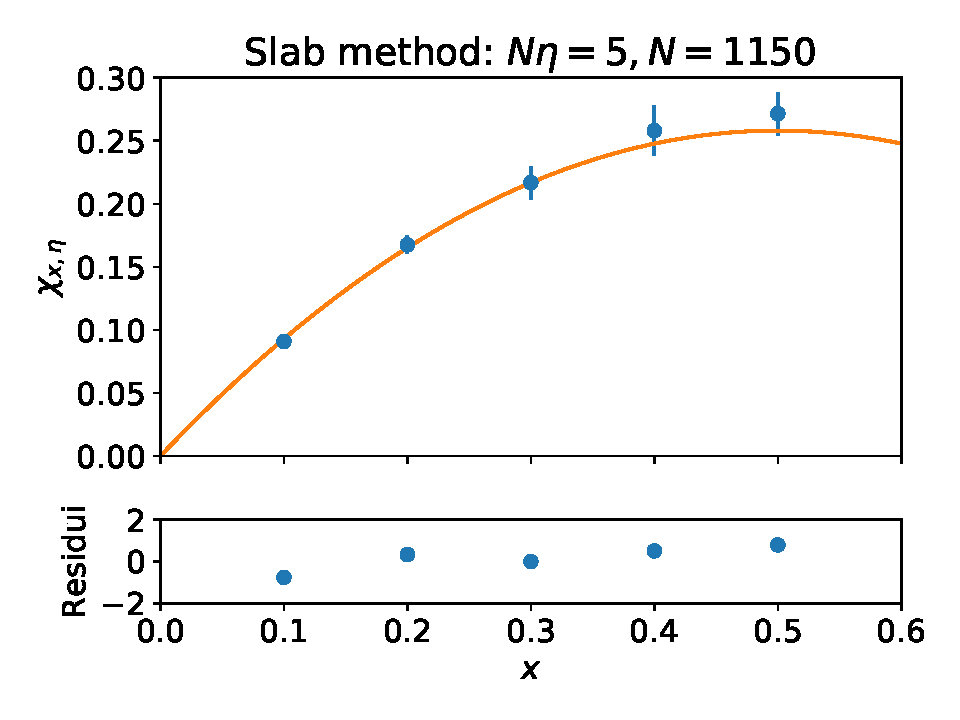
\includegraphics[width=0.5\textwidth]{figure/slab_fit_5_1150.pdf}} \\
        \subfloat[$N = 1250$]{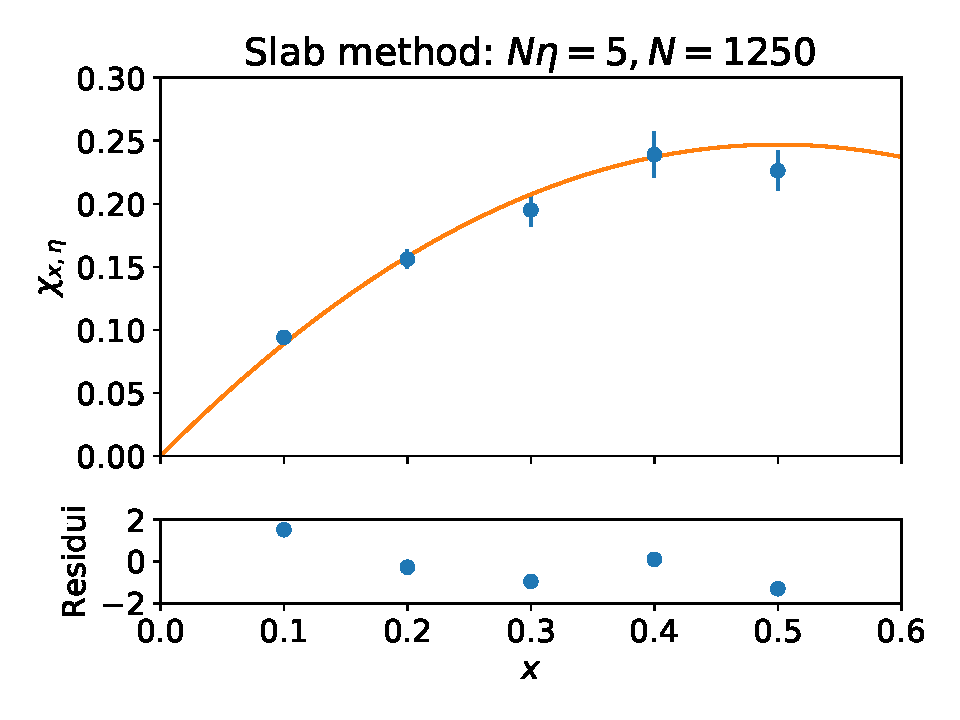
\includegraphics[width=0.5\textwidth]{figure/slab_fit_5_1250.pdf}} 
        \subfloat[$N = 1350$]{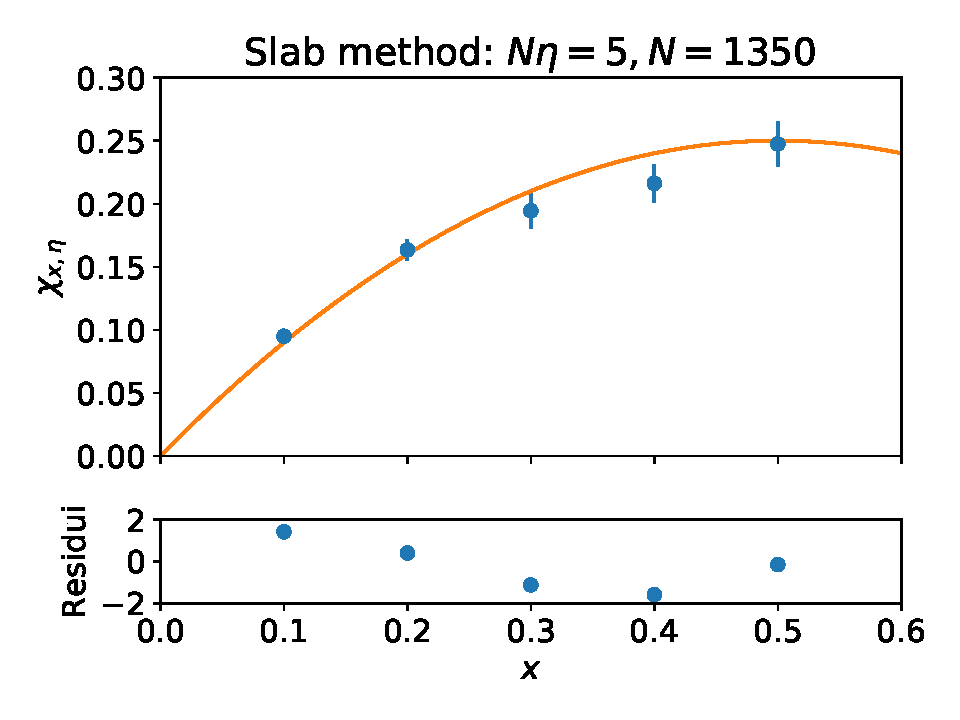
\includegraphics[width=0.5\textwidth]{figure/slab_fit_5_1350.pdf}} \\
        \subfloat[$N = 1500$]{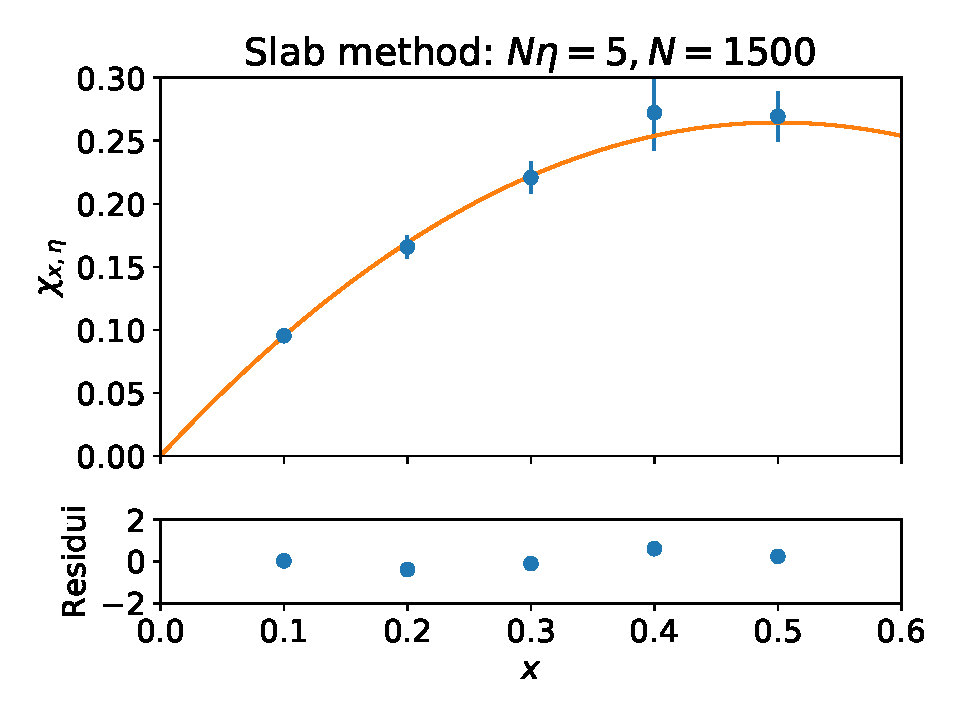
\includegraphics[width=0.5\textwidth]{figure/slab_fit_5_1500.pdf}} 
        \subfloat[Limite al continuo]{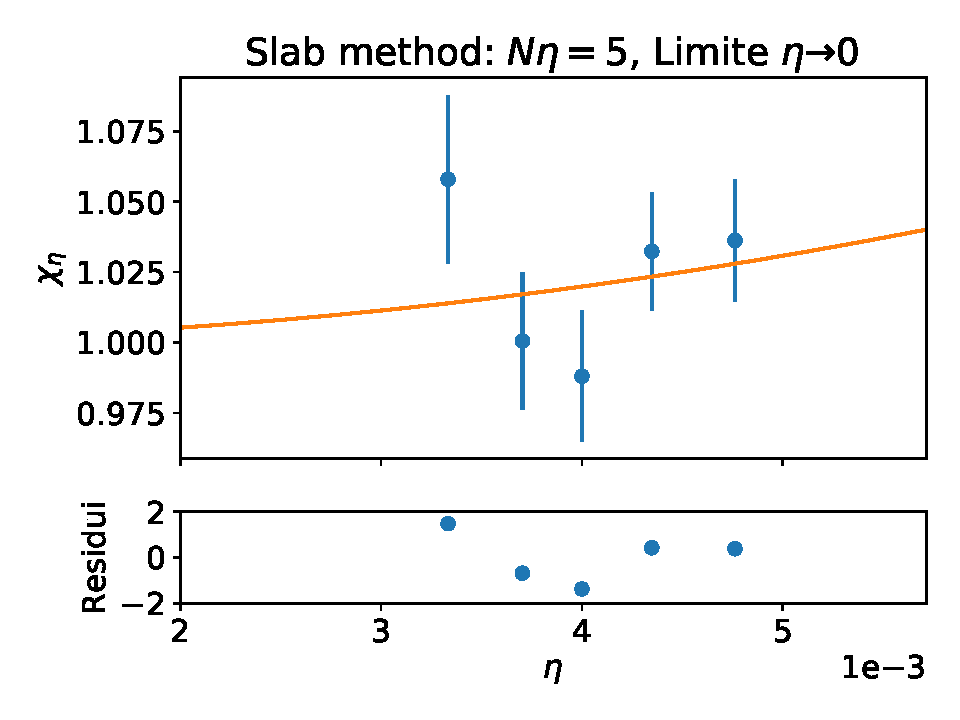
\includegraphics[width=0.5\textwidth]{figure/slab_fit_5_continuum.pdf}}
        \caption{Misura della suscettività topologica per $\beta = 5$ con lo slab method.}
        \label{fig:top_slab}
    \end{figure}

    
    
   
    
    \section{Studio dello spettro e funzioni di correlazione}
    
    Poiché conosciamo già lo spettro del sistema, possiamo immediatamente dire che le osservabili $O_n \equiv a^n + {a^\dagger}^n$ connettono lo stato fondamentale con gli stati del livello energetico n-esimo.
    
    Di conseguenza, possiamo dire che, nel limite $\beta \to \infty$, 
    %
    \begin{equation}
        C_n (\tau) \equiv \avg{ O_n(\tau)O_n(0) }_\beta - \avg{O_n}^2_\beta \sim A e^{-(E_n - E_0) \tau}
        \label{eqn:correlator}
    \end{equation}
    %
    Possiamo quindi calcolare il gap tra il livello n-esimo e il fondamentale studiando l'andamento delle funzioni di correlazione. 
    
    Questo non sembra particolarmente utile: abbiamo utilizzato il fatto che conosciamo già lo spettro del sistema! Tuttavia, questo può essere usato come punto di partenza per studiare il sistema in presenza di un potenziale esterno (purché l'azione sia definita positiva). 
    
    Studieremo il correlatore associato al primo livello energetico:
    %    
    \begin{equation}
         C_1 (\tau) \equiv \avg{\cos 2\pi x(\tau) \cos 2\pi x(0)}_\beta 
    \end{equation}
    %
    Questo correlatore è già connesso.
    
    \subsection{Simulazione numerica}

    Sono state effettuate varie simulazioni con l'algoritmo non locale, con $\beta = 5$, N = 750, 850, 950, 1000, 1100, 1200, 1300, 1400, 1500, ognuna da $10^6$ misure, una ogni 10 spazzate. Sono state scartate le prime $2 \cdot 10^5$ misure per termalizzazione. 
    
    Per ogni N, è stato stimato il gap di energia $\Delta E_1(N)$ con un fit numerico all'equazione \ref{eqn:correlator}, per $\tau < 0.1$. Questo è possibile perché $\cos 2\pi x$ connette lo stato fondamentale solo con il primo livello eccitato. Se non fosse stato così, sarebbe stato necessario studiare il comportamento asintotico del correlatore (lontano da 0 e da $\beta$).
    
    Gli errori su $\Delta E_1(N)$ sono stati stimati con un algoritmo Bootstrap a 100 campioni, con blocchi di dimensione $10^3$. In linea di principio, bisognerebbe studiare la stima dell'errore al variare delle dimensioni del blocco e del numero di campioni. A causa di limitazioni tecniche\footnote{Un banco di RAM ha misteriosamente smesso di funzionare}, questo non è stato possibile in modo rigoroso. Tuttavia, alcuni tentativi poco costosi dal punto di vista computazionale hanno mostrato che l'errore non varia in maniera sostanziale per blocchi di dimensione $10^3$ --- $10^4$ per $N = 850$.
    
    In figura \ref{fig:energy_continuum} è riportata l'analisi del limite al continuo dell'energia del primo livello $\Delta E_1$. Il fit numerico ad una funzione $\Delta E_1(\eta) = \Delta E_1 + k\eta^2$ fornisce un valore $\Delta E_1 = 19.742(20)$, da confrontare con il valore teorico $\Delta E_1 = 2\pi^2 \simeq 19.739\dots$. 
    
    Si ha un ottimo accordo con la teoria, con un $\chi^2 / \text{ndof} \simeq 0.81$.
    
    È interessante vedere cosa sarebbe successo se non fosse stato usato il Bootstrap per stimare gli errori sul fit. Nella figura \ref{fig:energy_continuum_wrong} mostriamo l'analisi del limite al continuo per $\Delta E_1$, dove gli errori sui singoli punti sono stati stimati attraverso le usuali procedure di best-fit per misure indipendenti. 
    
    Il risultato di questo fit ``sbagliato'' è apparentemente soddisfacente: $\Delta E_1 = 19.7385(45)$, in buon accordo con il valore teorico. Tuttavia, otteniamo un $\chi^2 / \text{ndof} \simeq 5.7$, segno che gli errori sono stati sottostimati. Infatti, così come in una simulazione $(N, N\eta)$ le varie misure di $C(\tau)$ a $\tau$ fissato non sono fra loro indipendenti, non lo sono neanche le varie misure di $C(\tau)$ al variare di $\tau$.   
    
    
    
    \begin{figure}[h!]
        \centering
        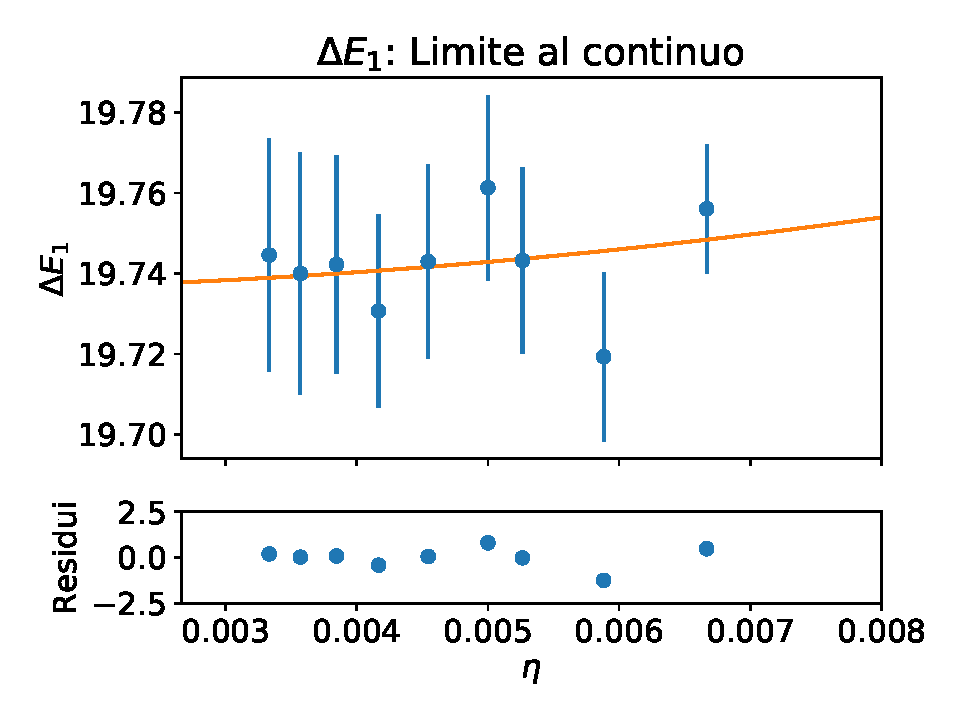
\includegraphics[width=0.6\textwidth]{figure/energy_continuum_5.pdf}
        \caption{Misura dell'energia del primo livello: limite al continuo. Gli errori sui singoli dati sono stati stimati con il Bootstrap}
        \label{fig:energy_continuum}
    \end{figure}
    
    \begin{figure}[h!]
        \centering
        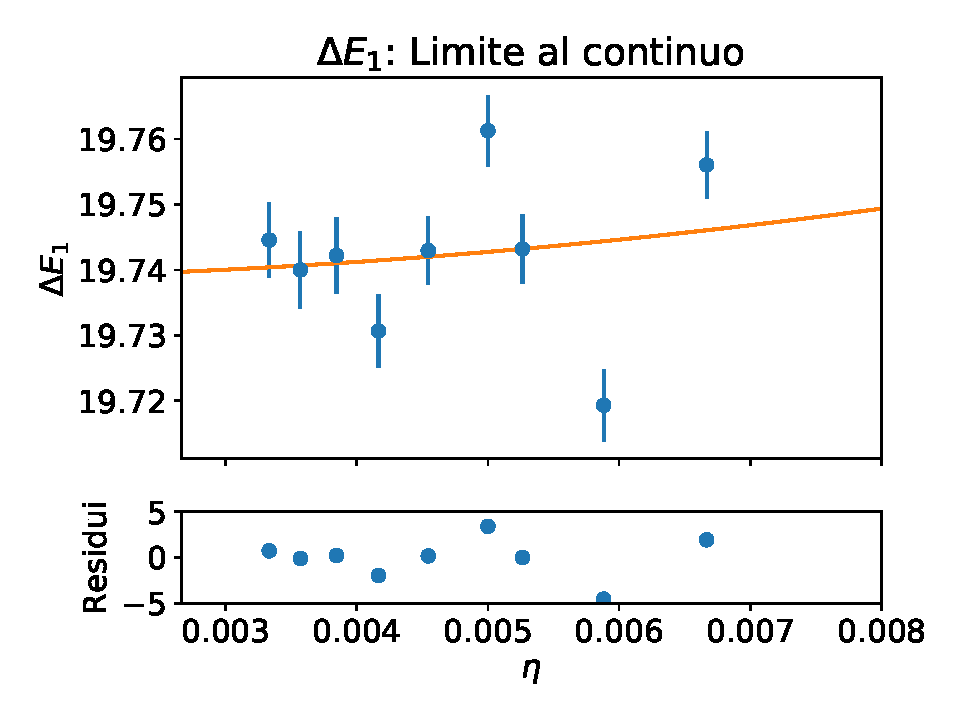
\includegraphics[width=0.6\textwidth]{figure/energy_continuum_5_wrong.pdf}
        \caption{Misura dell'energia del primo livello: limite al continuo. Gli errori sui singoli dati sono stati stimati con gli usuali metodi di best-fit per misure indipendenti. Questa condizione non è verificata, e gli errori sono fortemente sottostimati.}
        \label{fig:energy_continuum_wrong}
    \end{figure}



    

    
\end{document}
